\StartOf{Lecture 10}

\Today{(0) Activity for Binary 1-D Decision Theory; (1) Random Processes for Noise (2) Gaussian Random Vectors }

\announcements{
\begin{itemize}
\item Reading: Today: Rice 4.4-4.5; Mon: Rice 6.1, 6.2
\item HW 4 due today at 11:59pm, Project 3 due Mon at 11:59pm
\item HW 5 due Wed at 11:59pm.  When should I post solutions? 
\item Exam 1 is Mon March 2 in class.
\end{itemize}
}

\subsection{Activity}

To motivate detection theory, think of the following 1-D binary baseband PAM system.  The transmitter sends either $s_0(t) = a_0p(t)$ or $s_1(t) = a_1p(t)$.  The receiver correlates the received signal with $p(t)$ and measures $X = a_0 + N$ or $X=a_1 + N$.  Your receiver decides based on $X$ what symbol was sent.  

In the game version of this real-world problem, you will work in a team and compete against other teams. Your team must choose a threshold, where if $X<$ this threshold, your receiver will decide that $s_0(t)$ was sent; and if $X>$ the threshold, it will decide $s_1(t)$ was sent.  In Matlab, I will generate random symbols and random noise, and calculate based on your threshold, and 100 trials, what your number of errors is.  The team with the fewest errors wins.

  \begin{figure}[htbp]
    \centerline{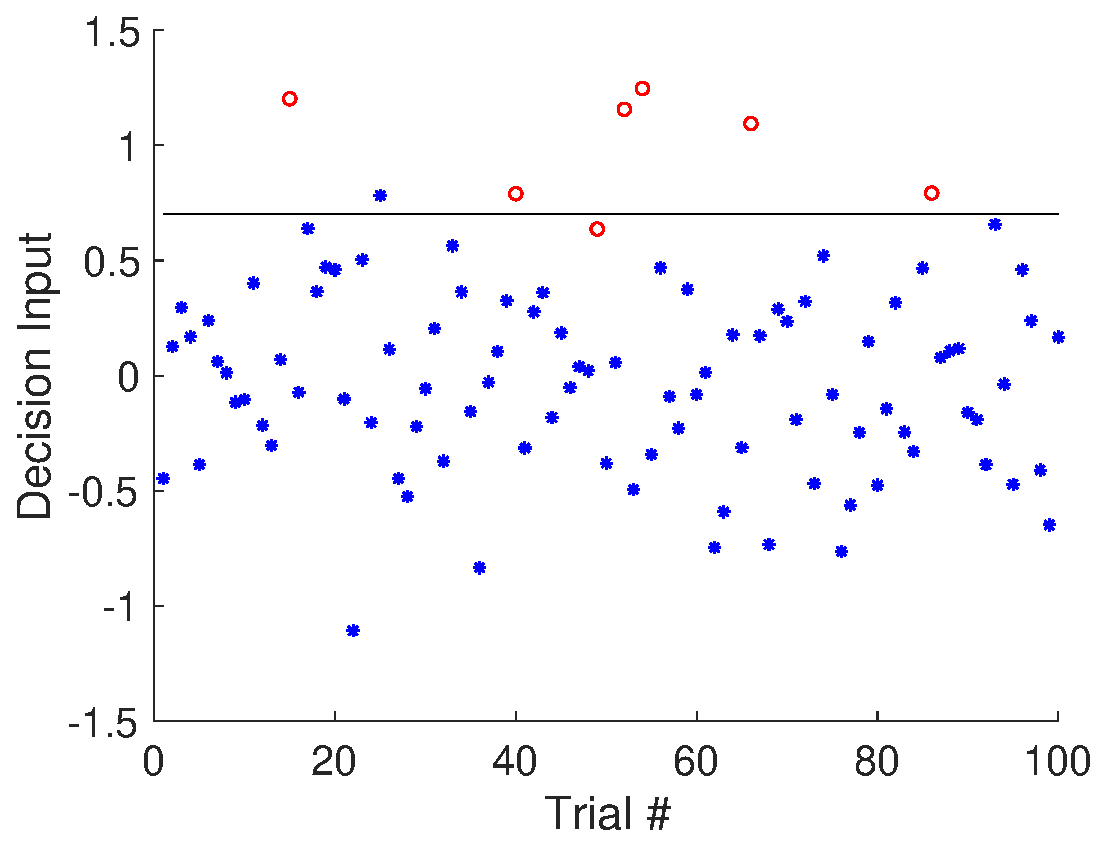
\includegraphics[width=2.4in]{../images/LectureActivitySymbolErrors.eps} }
    \caption{Activity example for threshold $= 0.7$, $a_0=0$, $a_1=1$, $\sigma_w=0.4$, $\PR{H_0}=0.9$, and 100 trials.  There are a total of 2 errors.}
    \label{F:LectureActivitySymbolErrors}
  \end{figure}


\section{Detection with Multiple Symbols}

When we only had $s_0(t)$ and $s_1(t)$, we saw that our decision was
based on which of the following was higher:
\[
  f_{X|H_0}(x| H_0) \PR{H_0} \quad \mbox{and} \quad f_{X|H_1}(x| H_1) \PR{H_1}
\]

For $M$-ary signals, we'll see that we need to consider the highest
of all $M$ possible events $H_m$,
\begin{eqnarray}
  H_0: && r(t) = s_0(t) + w(t) \nonumber \\
  H_1: && r(t) = s_1(t) + w(t) \nonumber \\
  \cdots && \cdots \nonumber \\
  H_{M-1}: && r(t) = s_M(t) + w(t) \nonumber
\end{eqnarray}
which have joint probabilities,
\begin{eqnarray}
  H_0: && f_{X|H_0}(x| H_0) \PR{H_0} \nonumber \\
  H_1: && f_{X|H_1}(x| H_1) \PR{H_1} \nonumber \\
  \cdots && \cdots \nonumber \\
  H_{M-1}: && f_{X|H_{M-1}}(x| H_{M-1}) \PR{H_{M-1}} \nonumber
\end{eqnarray}
A similar derivation to the one we did for binary 1-D Bayesian detection would show that the region $R_i$ in which it is optimal to decide $H_i$ is for all $X$ such that its joint probability is highest, that is,
\[
R_i = \left\{ X \mbox{ s.t. } f_{X|H_i}(x| H_i) \PR{H_i} > f_{X|H_j}(x| H_j) \PR{H_j} \mbox{ for all } j\neq i \right\}
\]

For this class, we'll usually consider the case of equally probable signals.  (While equi-probable signals is sometimes not the case for
$M=2$ binary detection, it is very rare in higher $M$ communication
systems because it is easy for communications systems designers to encode the data so that each symbol is equally likely to be transmitted.)  If $\PR{H_0} = \cdots = \PR{H_{M-1}}$ then we only need to find the $i$ that makes the likelihood $f_{X|H_i}(x| H_i)$ maximum, that is, maximum likelihood detection.
\[
  \mbox{Symbol Decision} = \arg \max_i f_{X|H_i}(x| H_i)
\]
For Gaussian (conditional) r.v.s with equal variances $\sigma_w^2$,
it is better to maximize the log of the likelihood rather than the likelihood directly, so
\[
  \log f_{X|H_i}(x| H_i) =  -\frac{1}{2}\log (2\pi \sigma_w^2)  - \frac{(x-a_i)^2}{2\sigma_w^2}
\]
This is maximized when $(x-a_i)^2$ is minimized.  Essentially, this
is a (squared) distance between $x$ and $a_i$.  So, the decision is,
find the $a_i$ which is closest to $x$.

The decision between two neighboring signal vectors $a_i$ and
$a_{i+1}$ will be
\[
 r  \decision{H_{i+1}}{H_i} \gamma_{i,i+1} = \frac{a_i + a_{i+1}}{2}
\]


As an example:  4-ary PAM.  See Figure
\ref{F:4AryPAM-DecisionThresholds}.

  \begin{figure}[htbp]
    \centerline{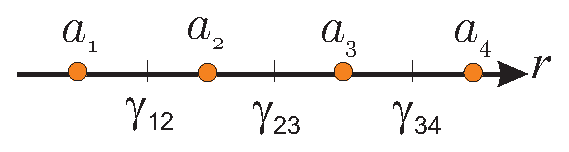
\includegraphics[width=2.4in]{../images/4AryPAM-DecisionThresholds.eps} }
    \caption{Signal space representation and decision thresholds for 4-ary PAM.}
    \label{F:4AryPAM-DecisionThresholds}
  \end{figure}


\section{Random Processes for Noise}

In order to study how noise affects communications receivers, we need to recall some background in the analysis of random processes.  A \emph{random process} $X(t)$ is a random function of continuous time $t$. (A \emph{random sequence} $X(n)$ is a sequence of random variables indexed by time index $n$.)  

The physics of thermal noise says that it has power spectral density that is approximately $kT_e$ where $k=1.3807\times 10^{23}$ J/K is Boltzmann's constant and $T_e$ is called the ``effective noise temperature'', which is proportional to the temperature of what the antenna is pointing at, and multiplied by a factor related to noise amplification within the receiver.  $T_e$ is a temperature in Kelvin.  This constant $kT_e$ is constant across the frequencies we use for communications system.  At room temperature, the power spectral density of thermal noise goes to zero at frequencies above $10^{13}$ Hz, that is, 10 Terahertz or 10,000 GHz.  This is orders of magnitude above frequencies at which most communications signals are sent.  The Rice book (4.5.2) has a good analysis of
the physics of thermal noise.  In short, the physics says that the PSD is flat in the bands we use, and that it is zero mean.

One of the most important and surprising results from random processes is that the autocorrelation function and the power spectral density are Fourier transform pairs, given certain conditions.  This helps us figure out how noise affects receivers, as we show next. 

\subsection{Autocorrelation and Power Spectral Density}


\Definition{Mean Function}{The mean function of the random
process $X(t)$ is 
\[
  \mu_X(t) = \E{}{X(t)}
\]
}
Note the mean is taken over all possible realizations of $X(t)$.  If you record one signal over all time $t$, you don't have anything to average to get the mean function $\mu_X(t)$.

\Definition{Autocorrelation Function}{ The autocorrelation function
of a random process $X(t)$ is
\[
  R_X(t, \tau) = \E{}{X(t) X(t - \tau)}
\]
The autocorrelation of a random sequence $X(n)$ is
\[
  R_X(n, k) = \E{}{X(n) X(n - k)}
\]
}

\Definition{Wide-sense stationary (WSS)}{ A random process is
wide-sense stationary (WSS) if
\begin{enumerate}
  \item $\mu_X = \mu_X(t) = \E{}{X(t)}$ is independent of $t$.
  \item $R_X(t, \tau)$ depends only on the time difference
  $\tau$ and not on $t$.  We then denote the
  autocorrelation function as $R_X(\tau)$.
\end{enumerate}
A random process is wide-sense stationary (WSS) if
\begin{enumerate}
  \item $\mu_X = \mu_X(n) = \E{}{X(n)}$ is independent of $n$.
  \item $R_X(n, k)$ depends only on $k$ and not on $n$.  We then denote the
  autocorrelation function as $R_X(k)$.
\end{enumerate}}
\textbf{The power of a signal is given by $R_X(0)$.}


\paragraph{Power Spectral Density}

The power spectral density $S_X(f)$ is a positive real-valued function equal to the density of power in a random process $X(t)$ near the frequency $f$.  It has units of Watts / Hz.  The (average) power between two frequencies $f_1$ and $f_2$ is the integral of $S_X(f)$ from $f_1 < f < f_2$. 

We know from random processes:  For a WSS random process $X(t)$ (and for a random
sequence $X(n)$) that its power spectral density can be computed as,
\begin{eqnarray}
  S_X(f) &=& \Fourier{R_X(\tau)} \nnn
  S_X(e^{j\Omega}) &=& \DTFT{R_X(k)} \nn
\end{eqnarray}

\Example{What is the autocorrelation function for thermal noise?}

We know from physics that thermal noise has constant power spectral density, and that the random process is WSS.  As Rice says ``for historical reasons this constant value is designated $N_0/2$''.  In this case, what is the autocorrelation function $R_w(\tau)$?

\Solution{
We're given $S_w(f) = N_0/2$.  The relationship is:
\[
S_X(f) = \Fourier{R_X(\tau)} 
\]
So 
\[
R_X(\tau) =\IFourier{S_X(f)} = \IFourier{N_0/2}
\]
But $N_0/2$ is just a constant.  Looking at a Fourier transform table, the solution is
\[
R_X(\tau) = \frac{N_0}{2} \delta (\tau).
\]
}

\subsection{Uncorrelated Noise}

A random sequence $X(n)$ is an \emph{uncorrelated noise} sequence if it is WSS and has autocorrelation function
\[
  R_X(k) = \E{}{X(n)X(n-k)} = \sigma^2 \delta(k)
\]
This says that each element of the sequence $X(n)$  is uncorrelated with $X(m), m\neq n$.

A random process $X(t)$ is an \emph{uncorrelated noise} random process if it is WSS and has autocorrelation function
\[
  R_X(\tau) = \E{}{X(t)X(t-\tau)} = \sigma^2 \delta(\tau)
\]
Again, this says that the value of $X(t)$  is uncorrelated with $X(t'), t'\neq t$.


This noise random process is referred to in textbooks as `white noise' because it has equal parts of every frequency (analogy to light).  But as I've mentioned before, black and gray also are constant in the frequency domain, so calling it `white' is arbitrary.  A more precise name is \emph{uncorrelated noise}.

Note that describing a random process / sequence as ``uncorrelated'' does NOT say that the distribution of its samples are Gaussian.  In order to specify that, we call it \emph{uncorrelated Gaussian noise}.  We typically model thermal noise as additive uncorrelated Gaussian noise (AUGN).  That is, it adds to the received signal.








\subsection{Noise in Correlation Receiver}

Previously, we had said that $r(t)$ was equal to the transmitted signal $s(t)$ plus noise:
\[
 r(t) = s(t) + w(t)
\]
As implied, we consider $w(t)$ to be uncorrelated and Gaussian with zero mean and PSD $S_W(f) = N_0/2$, or equivalently, $R_W(\tau) = N_0/2 \delta(\tau)$.  

What is the output of the correlation receiver?  Recall $x_k$ is defined as $\langle r(t), \phi_k(t) \rangle$, or
\begin{eqnarray}
  x_k &=& \int_{-\infty}^\infty r(t) \phi_k(t) dt
      \nonumber \\
    &=& \int_{-\infty}^\infty [s_i(t) + w(t)] \phi_k(t) dt
      \nonumber \\
    &=& a_{i,k} + \int_{-\infty}^\infty w(t) \phi_k(t) dt
      \nonumber \\
    &=& a_{i,k} + w_k
      \nonumber
\end{eqnarray}
where we define
\[
 w_k = \langle w(t), \phi_k \rangle = \int_{-\infty}^\infty w(t) \phi_k(t) dt.
\]

What can we know about $w_k$?  What are the mean and covariance of $\{w_k\}$?  For practice, prove that: 1) $w_k$ are all zero mean; and 2) the correlation of $w_k$ and $w_m$ is zero unless $k=m$, and in that case, is equal to $N_0/2$.  

\Solution{
First, $w_k$ is zero mean:
\[
  \E{}{w_k} = \int_{-\infty}^\infty \E{}{w(t)} \phi_k(t) dt = 0
\]
Next we can show that $w_1, \ldots, w_N$ are i.i.d. by calculating
the autocorrelation $R_w(m,k)$.
\begin{eqnarray}
  R_w(m,k) &=& \E{}{w_k w_m}
      \nonumber \\
    &=& \int_{t=-\infty}^\infty \int_{\tau=-\infty}^\infty \E{}{w(t) w(\tau)} \phi_k(t) \phi_m(\tau) d\tau dt
      \nonumber \\
    &=& \int_{t=-\infty}^\infty \int_{\tau=-\infty}^\infty \frac{N_0}{2}\delta(t-\tau) \phi_k(t) \phi_m(\tau) d\tau dt
      \nonumber \\
    &=& \frac{N_0}{2} \int_{t=-\infty}^\infty \phi_k(t) \phi_m(t) dt
      \nonumber \\
    &=& \frac{N_0}{2} \delta(k-m) = \pdfarray{\frac{N_0}{2}}{m=k}
      \nonumber
\end{eqnarray}
}

Is $w_k$ Gaussian?  Yes -- an integral is a linear operation, and any linear function of a Gaussian random process is also Gaussian.  

Are $\{w_k\}$ independent?  Yes -- for Gaussian random variables, a covariance of zero implies independent.  

Since the noise components are independent, then $x_k$ (the sum of $a_{i,k}$ and $w_k$) are also
Gaussian and independent. Why? Because $a_{i,k}$ is a deterministic constant, and thus $x_k$ are Gaussian with mean $a_{i,k}$.  But that change in mean doesn't change the autocovariance function. 

What is the pdf of $\mbx = [x_0, \ldots, x_K]^T$?

\Solution{ 
\[
 f_{X_k}(x_k) = \frac{1}{\sqrt{2\pi (N_0/2)}} e^{-\frac{(x_k - a_{i,k})^2}{2(N_0/2)}}
\]
And, since the $\{x_k\}$ are independent, the joint pdf of all of them is the product of the marginal pdfs:
\begin{eqnarray}
 f_{\mbx}(\mbx) &=& \prod_{k=1}^K f_{X_k}(x_k) \nonumber \\
   &=& \prod_{k=1}^K \frac{1}{\sqrt{2\pi (N_0/2)}} e^{-\frac{(x_k - a_{i,k})^2}{2(N_0/2)}}
     \nonumber \\
   &=& \frac{1}{[2\pi (N_0/2)]^{K/2}} e^{-\frac{\sum_{k=1}^K (x_k - a_{i,k})^2}{2(N_0/2)}}
     \nonumber
\end{eqnarray}
}

\subsection{Gaussian Random Vectors}

\Definition{Multivariate Gaussian R.V.}{An $n$-length R.V. $\mbX$
is multivariate Gaussian with mean $\mu_\mbX$,  and covariance
matrix $C_\mbX$ if it has the pdf,
\[
f_\mbX(\mbx) = \frac{1}{\sqrt{(2\pi)^n \mbox{det}(C_\mbX)}}
  \exp \left[ -\frac{1}{2}(\mbx-\mu_\mbX)^T  C_\mbX^{-1}
  (\mbx-\mu_\mbX) \right]
\]
where $\mbox{det}()$ is the determinant of the covariance matrix, and
$C_\mbX^{-1}$ is the inverse of the covariance matrix. }

\textbf{Any linear combination of jointly Gaussian random variables
is another jointly Gaussian random variable.}  For example, if we
have a matrix $A$ and we let a new random vector $\mbY = A \mbX$,
then $\mbY$ is also a Gaussian random vector with mean $A\mu_\mbX$
and covariance matrix $A C_\mbX A^T$.

If the elements of $\mbX$ were independent random variables, the pdf
would be the product of the individual pdfs (as with any random
vector) and in this case the pdf would be:
\[
f_\mbX(\mbx) = \frac{1}{\sqrt{(2\pi)^n \prod_i \sigma_i^2}}
  \exp \left[ -\sum_{i=1}^n \frac{(x_i-\mu_{X_i})^2}{2\sigma_{X_i}^2}  \right]
\]

Section 4.3 spends some time with 2-D Gaussian random vectors, which
is the dimension with which we spend most of our time in this class.
